
\section{Disegni di Studio}

\subsection{La ricerca scientifica}


Il primario interesse dei medici è il beneficio del pz e della comunità.
Come ci si arriva? È un processo lungo, che parte dalla ricerca
scientifica. Con questa si fa un ``focus on the bigger picture'', ovvero
si cerca di mettere in un contesto ciò che stiamo cercando con una
prospettiva più macroscopica. Per mezzo di questo di arriva al beneficio
del pz, questo processo è come la ricerca scientifica e nello specifico
la ricerca epidemiologica supporta il beneficio del pz nella clinica di
tutti i giorni.
\begin{figure}[!ht]
\centering
	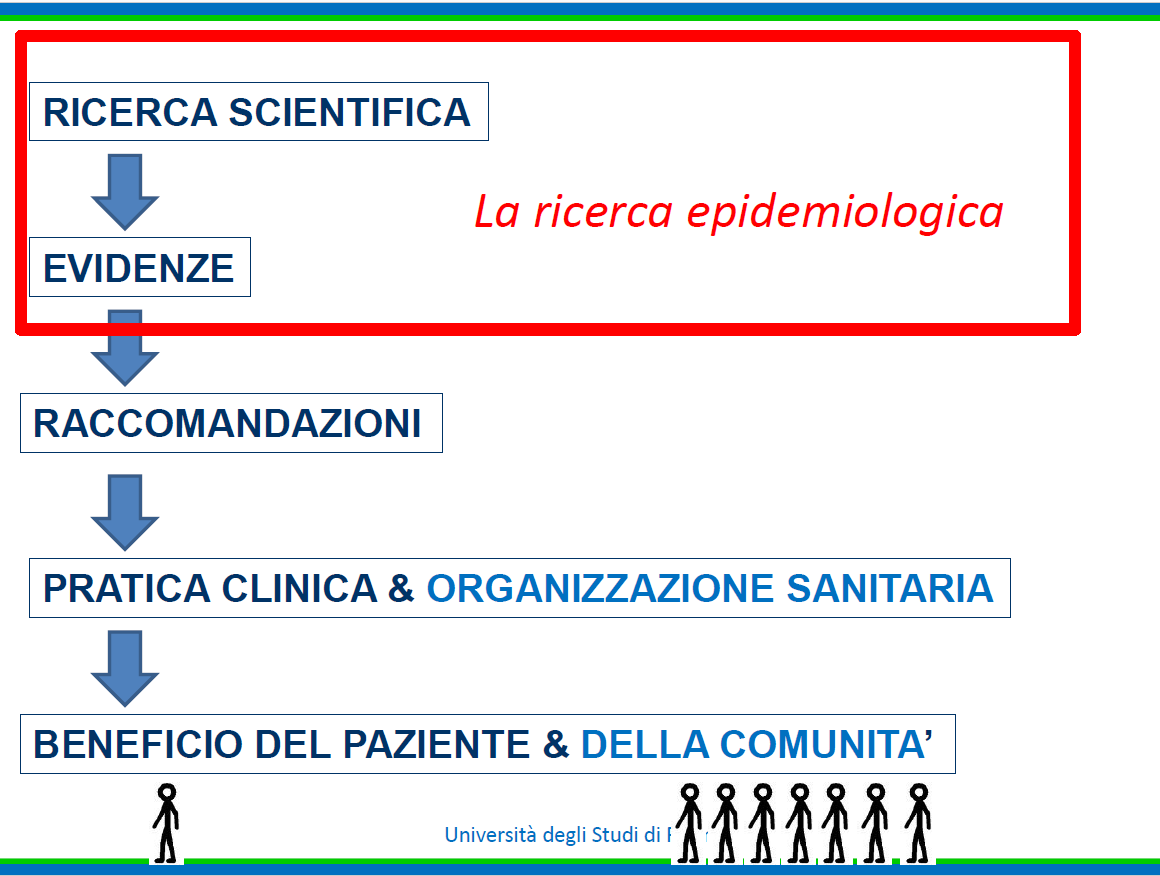
\includegraphics[width=0.8\textwidth]{04/image1.png}
	\end{figure}




\emph{Ricerca scientifica focus on the bigger picture beneficio del pz}

Vedremo quindi quali sono gli step di questo processo.

Ci sono ricerche scientifiche di vari tipi, qui ci si concentra sulla
ricerca epidemiologica.

\subsubsection{La ricerca epidemiologica}

La ricerca scientifica permette di arrivare ad \textbf{evidenze}, quindi
tesi supportate da ricerche dati su popolazioni.

Le evidenze vengono utilizzate per produrre \textbf{raccomandazioni},
come le linee guida.

Dalle linee guida si può fare pratica clinica ed organizzazione
sanitaria basata sulle evidenze e si raggiunge il fine ultimo, che è il
\textbf{beneficio} \textbf{del pz e delle popolazioni.}

\emph{Ricerca scientifica evidenze raccomandazioni buona pratica clinica
beneficio pz e popolazioni}

Nell'ambito della ricerca biomedica ci sono 4 livelli:

\begin{itemize}
\item
  dimensione molecolare (biologia, immunologia)
\item
  dimensione dei tessuti e degli organi (istologia, anatomia patologica,
  quindi indagini di laboratorio sui tessuti)
\item
  dimensione dell'individuo (pratica clinica)
\item
  dimensione della popolazione (epidemiologia): questa è quella su cui
  ci si focalizza qui.
\end{itemize}

\paragraph{Epidemiologia }


L'epidemiologia si occupa della raccolta e analisi di \emph{dati di
popolazione} con un fine che può essere

\begin{itemize}
\item
  DESCRITTIVO: descrivere la distribuzione dei fenomeni sanitari (es.
  prevalenza a livello mondiale della malaria)
\item
  ANALITICO: indagare i determinanti delle malattie (il termine
  ``cause'' al posto di ``determinanti'' è un po' impreciso, ma può
  servire per ricordare il concetto)
\end{itemize}

Si delineano diversi stadi:

\begin{enumerate}
\def\labelenumi{\arabic{enumi}.}
\item
  Study design, ovvero il disegno, la progettazione dello studio
  epidemiologico
\item
  Raccolta dei dati
\item
  Analisi dei dati
\item
  Interpretazione dei dati
\end{enumerate}

{[}nel programma di epidemiologia sono previsti 4 argomenti: fonti dati,
disegni di studio, analisi dati, interpretazione dati{]}

\paragraph{Disegni di studio}


L'epidemiologia raccoglie dati di popolazione, come questi dati vengono
raccolti e organizzati è il disegno di studio.

Ad esempio si può fare un disegno di studio per dimostrare
l'associazione tra fumo di sigaretta e neoplasia polmonare. Sembra
banale, ma è stato dimostrato con studi epidemiologici. Il disegno
organizza i dati al fine di rispondere a determinati quesiti di ricerca,
in questo caso la correlazione fumo-tumore al polmone.

Caratteristiche dei disegni di studio:

\begin{itemize}
\item
  dipendono dal quesito di ricerca (obiettivo) dello studio
\item
  sono influenzati dalla \emph{fattibilità}

  \begin{itemize}
  \item
    disponibilità di risorse economiche
  \item
    aspetti etici
  \item
    tempo
  \end{itemize}
\item
  determinano l'analisi statistica
\end{itemize}

Perché è importante conoscere i diversi disegni di studio?

\textbf{1.} Pianificare il progetto di ricerca, ad esempio per chiedere
fondi o fare una tesi. La conoscenza dei diversi tipi di disegni di
studio vi permette di selezionare le popolazioni oggetto di studio, di
definire gli outcome di interesse, di raccogliere i dati che sono
necessari e pianificare il tipo di analisi.

\textbf{2.} Per individuare i limiti legati a ciascun disegno di studio,
che ne condizionano la solidità delle evidenze prodotte.

Questa è la piramide delle evidenze:

\begin{figure}[!ht]
\centering
	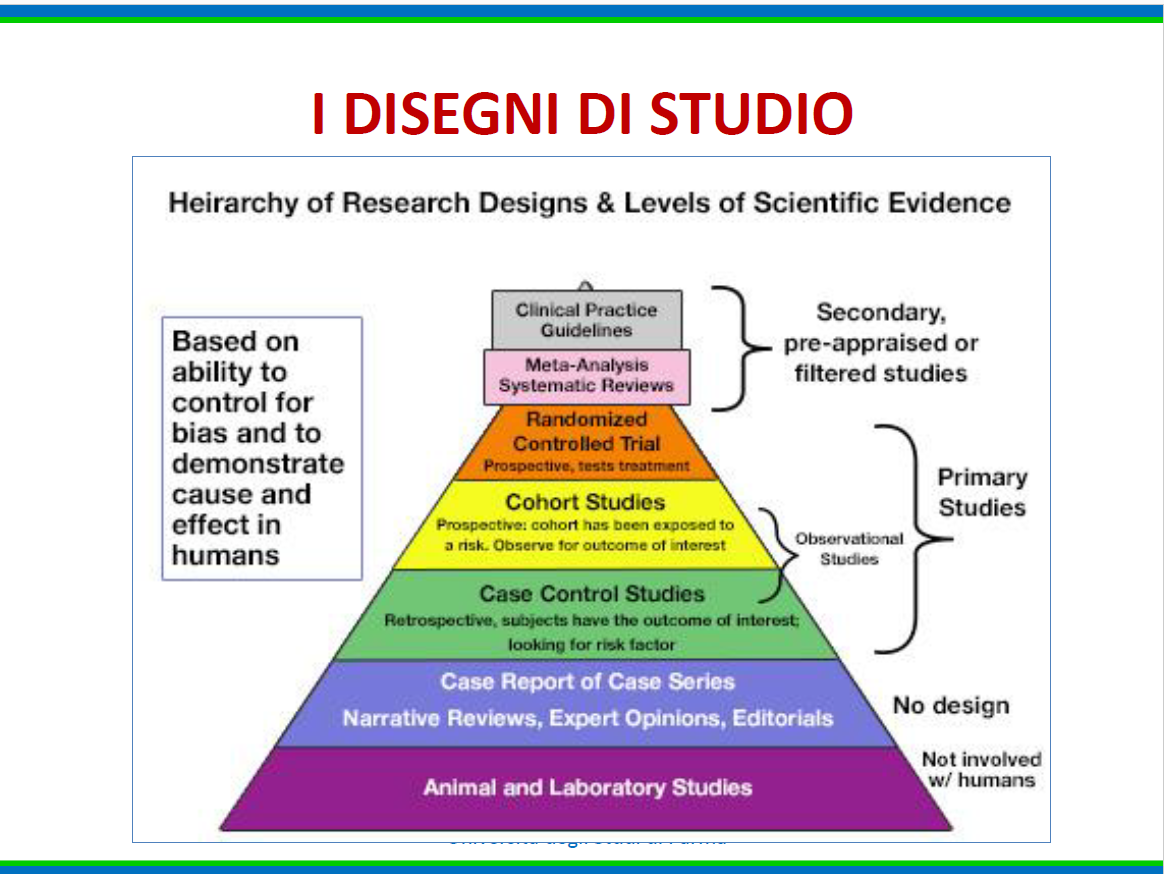
\includegraphics[width=0.8\textwidth]{04/image2.png}
	\end{figure}

Essa suddivide i disegni di studio in base al grado di solidità delle
evidenze, alla base ci sono gli studi più deboli e all'apice quelli più
solidi (meno limitate da bias ecc).

\subparagraph{Classificazione dei disegni di studio}


Ci sono diverse classificazioni, ma tutte li dividono su 3 livelli:

\begin{itemize}
\item
  \emph{fine}: descrittivo o analitico
\item
  \emph{dati}: aggregati o disaggregati
\item
  \emph{disegno}: osservazionali o sperimentali
\end{itemize}

dati

\emph{disaggregati}: di singoli individui

\emph{aggregati}: di gruppi di individui (ad esempio incidenza tumore
alla mammella in Emilia Romagna vs Toscana, confronta gruppi di
individui)

disegno (la più classica)

- \emph{osservazionali}: osservare i fenomeni e basta

- \emph{sperimentali}: viene introdotto ai fini della ricerca
l'esposizione, la terapia o l'intervento.

I più classici degli sperimentali sono i trials clinici, soprattutto
quelli che valutano l'efficacia dei farmaci.

\begin{figure}[!ht]
\centering
	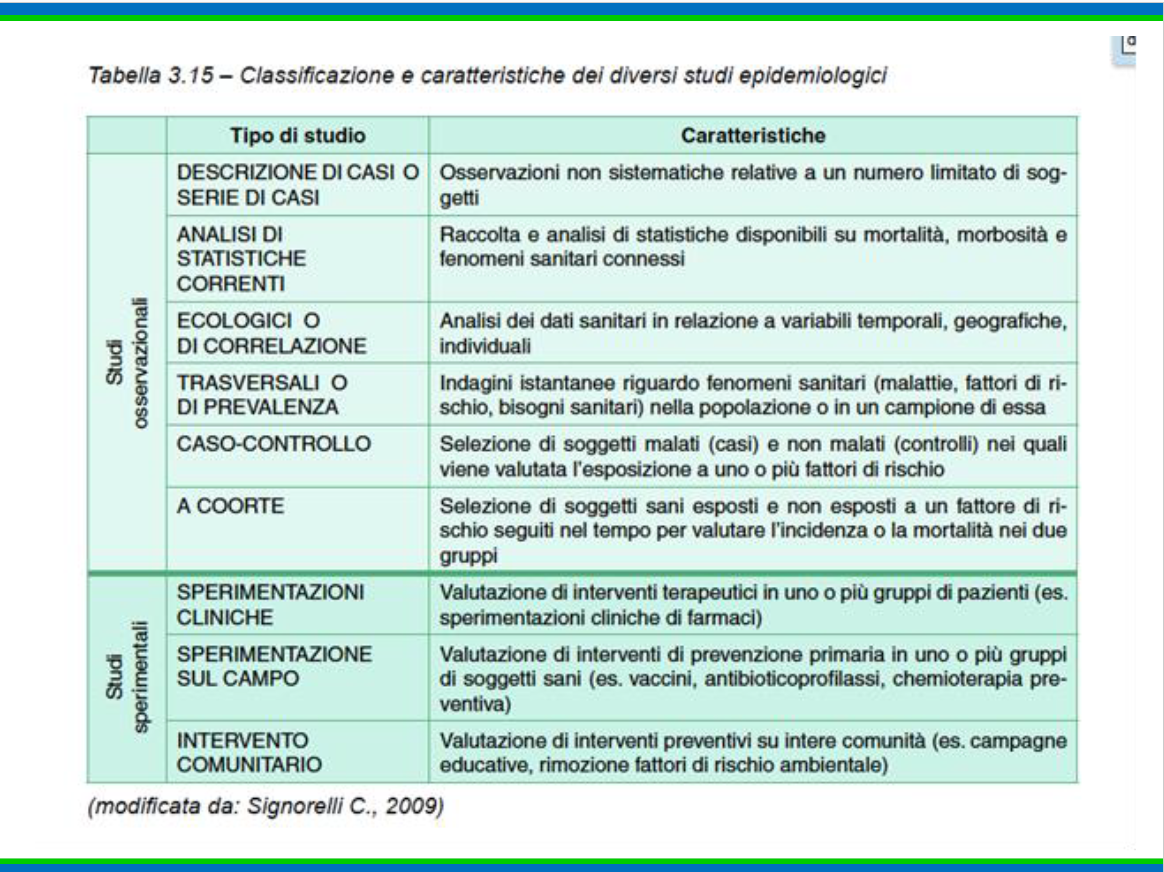
\includegraphics[width=0.8\textwidth]{04/image3.png}
	\end{figure}

\subparagraph{Studi osservazionali }


A) \textbf{Case report} (descrizione di casi clinici) e \textbf{Case
series} (serie di casi): osservazioni non sistematiche relative a un
numero limitato di soggetti.

\begin{enumerate}
\def\labelenumi{\arabic{enumi}.}
\item
  \textbf{Case report}: descrizione dettagliata di segni e sintomi e
  risultati di laboratorio di un caso singolo.
\end{enumerate}

Perché è utile? Potrebbe essere un caso particolarmente interessante che
può stimolare la riflessione. Di solito vengono pubblicati casi
eclatanti o particolarmente importanti.

\begin{enumerate}
\def\labelenumi{\arabic{enumi}.}
\item
  \textbf{Case series}: descrizione dettagliata di segni e sintomi e
  risultati di laboratorio di un numero limitato di casi (fino a 5
  casi).
\end{enumerate}

B) \textbf{Analisi di statistiche correnti}: studi descrittivi che usano
\emph{dati aggregati}, dati amministrativi, statistiche ricorrenti;
descrivono eventi sanitari per età, sesso, periodo, distribuzione
geografica.

Es. Incidenza di tubercolosi nel mondo. Dalla figura si vede come sia
maggiore in Sud Africa (blu scuro) rispetto Nord America ed Europa
(azzurro). A cosa ci può servire questo dato? Può essere utile a livello
politico sanitario per allocare risorse e per la programmazione di
interventi sanitari, quindi incide sull'organizzazione della sanità
pubblica.

\begin{figure}[!ht]
\centering
	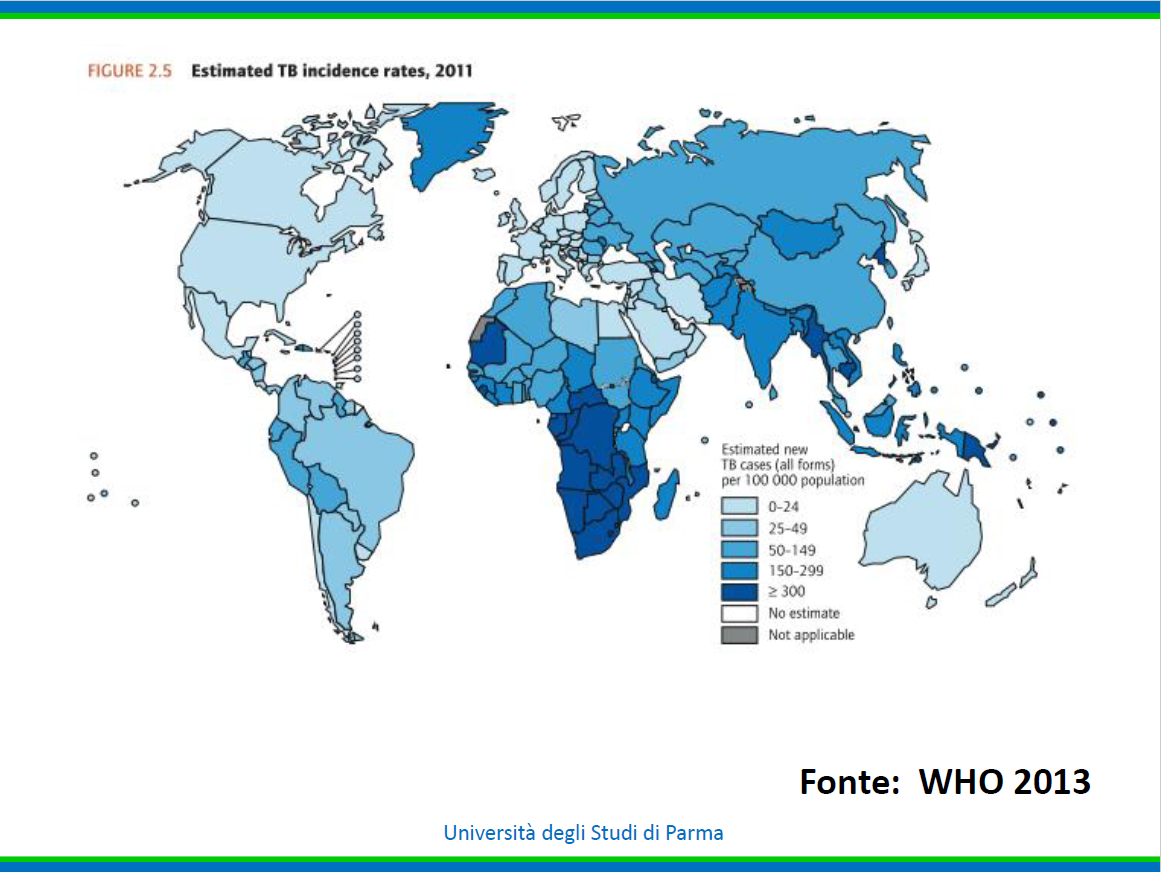
\includegraphics[width=0.8\textwidth]{04/image4.png}
	\end{figure}

C) \textbf{Studi ecologici o di correlazione}: utilizzano \emph{dati
aggregati} non solo per descrivere un fenomeno, ma anche per studiarne i
determinanti. Anche questi utilizzano dati provenienti da flussi
amministrativi e statistiche correnti.

Vengono fatti perché generalmente poco costosi e relativamente rapidi,
proprio perché utilizzano dati già disponibili, anche se hanno una serie
di limitazioni.

Riassumendo, studia l'associazione tra un'esposizione e un outcome,
utilizzando dati aggregati.

\emph{Ciò che fa sempre uno studio è studiare questa associazione tra
un'esposizione, ovvero un fattore di rischio, e un outcome, ovvero una
malattia.}

Es. studio pubblicato sul BMJ del 2014: ha come indicatori sanitari 170
paesi per tipo di economia e grado di democrazia.

\begin{figure}[!ht]
\centering
	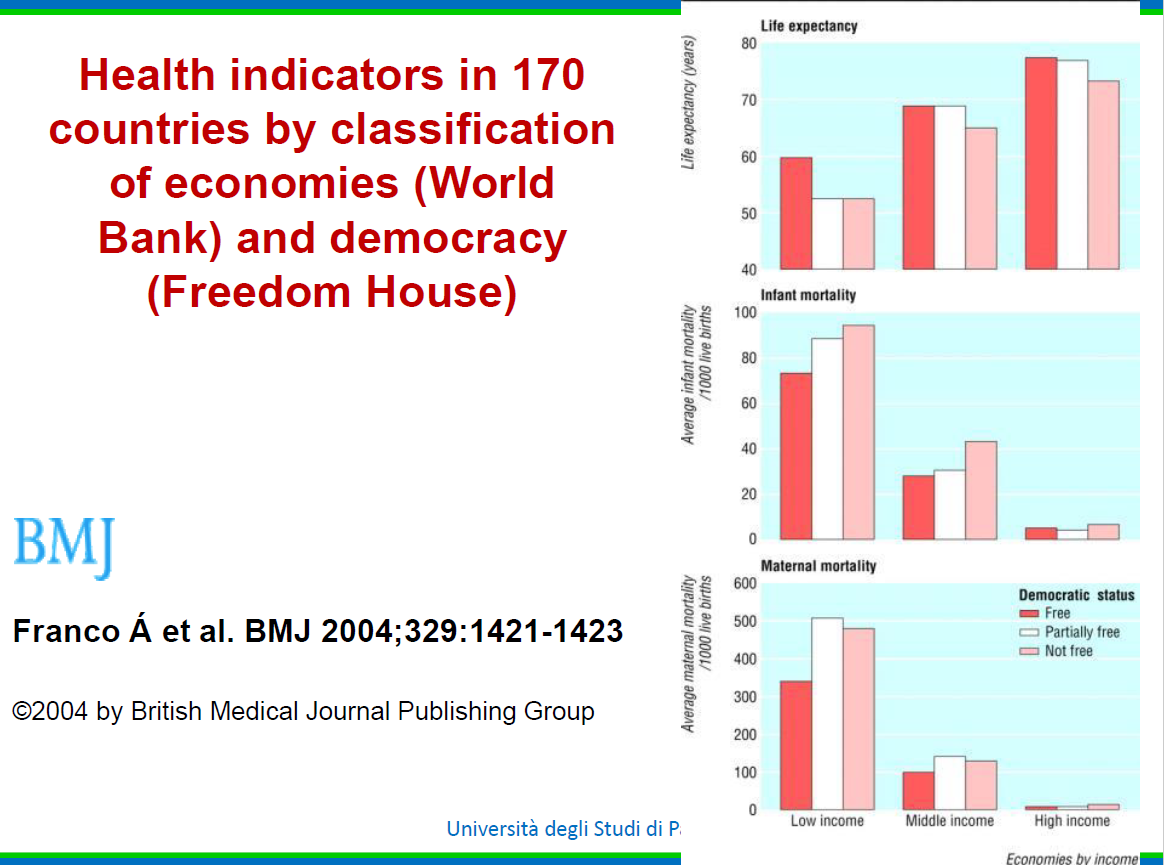
\includegraphics[width=0.8\textwidth]{04/image5.png}
	\end{figure}

Ci sono tre outcome: aspettativa di vita (grafico in alto), la mortalità
infantile (grafico in mezzo) e la mortalità materna (grafico in basso).

Esposizione: stato socioeconomico e livello di democrazia.

Il quesito di ricerca di partenza è: paesi con stato socio economico
diverso, hanno diversi outcomes sanitari?

Sono stati classificati 170 paesi con diverso gradi di esposizione (sono
dati aggregati, di interi paesi): poveri (gruppo di colonne a sinistra
di ciascuna delle tre tabelle), medi (colonne centrali), ricchi (a
destra).

Nel primo ad esempio l'aspettativa di vita aumenta in base allo stato
economico, è minore nei Paesi più poveri. Questa è la risposta al primo
quesito.

Poi i ricercatori hanno posto un secondo quesito: lo stato democratico
influenza questo outcome?

(stato democratico libero: colonne rosse; parzialmente libero: colonne
bianche; non libero: colonne rosa).

La mortalità infantile ad esempio per tutti i gradi di ricchezza è più
alta nei non democratici.

Quindi questo è un esempio di come dati aggregati di nazioni possano
essere usati per studiare l'associazione tra un' esposizione e un
outcome di interesse.

D) \textbf{Studi trasversali o di prevalenza}, cosiddetti \emph{studi
cross-sectional} (l'esempio più classico sono i questionari).

L'informazione è raccolta

\begin{enumerate}
\def\labelenumi{\arabic{enumi}.}
\item
  in un istante temporale definito, a un tempo 0 (es. numero di fumatori
  degli studenti di medicina anno 2016-2017), è uno studio
  \emph{trasversale}
\item
  dati da \emph{singoli individui}
\item
  dati su esposizione e/o outcomes (es. quesito ``vivere in un'area
  inquinata favorisce l'allergia?'': dove vive il soggetto=esposizione;
  è allergico=outcome)
\end{enumerate}

Gli studi trasversali sono tanto più validi e solidi, quanto più vengono
fatti su un campione che viene definito \emph{rappresentativo.}

Es. quesito: prevalenza del fumo nei ragazzi italiani di 23 anni. Per
avere la verità più assoluta si dovrebbero mandare questionari, lettere
via email a tutti i ragazzi italiani, ma questo per questioni di
fattibilità non è possibile (troppo dispendioso, troppo tempo ecc). Si
fa allora un \textbf{campione rappresentativo}: ci sono tecniche di
campionamento che mi permettono di selezionare un campione
rappresentativo.

Nella selezione è importante il concetto ``rappresentativo'': non si può
fare ad esempio solo sugli universitari, perché si avrebbero differenze
con i ragazzi lavoratori per abitudini. Se si fa solo sugli universitari
ovviamente poi si deve interpretare il dato considerando che non
riguarda tutti i ragazzi italiani: sarà rappresentativo della sola
popolazione universitaria.

La solidità dello studio trasversale è quindi legata alla
rappresentatività del campione che noi selezioniamo.

Es. Il The Lancet ha pubblicato nel 2013 un articolo sulle abitudini
sessuali inglesi, un esempio di studio cross-sectional. Perché ci può
essere un interesse di sanità pubblica? Per il controllo delle malattie
sessualmente trasmesse e l'educazione sessuale legata ai metodi
contraccettivi (in Inghilterra ci sono molte maternità giovanili non
volute).

Altro studio cross-sectional su Jama Neurology: la depressione (outcome)
in associazione alla disfunzione cognitiva (esposizione) misurata con
tecniche di neuroimaging negli ex giocatori di football professionisti.
Hanno comparato giocatori con impairment cognitivo e depressione e
giocatori con livello cognitivo normale e assenza di depressione.

Caratteristiche studi cross-secional:

\begin{itemize}
\item
  esposizione e outcome sono misurati \emph{allo stesso tempo}
\item
  relativamente rapidi ed economici
\end{itemize}

\begin{quote}
Limiti:
\end{quote}

\begin{itemize}
\item
  Reverse causality: siccome misura esposizione e outcome allo stesso
  tempo non permette di stabilire se l'esposizione viene prima o dopo
  l'outcome, non possiamo stabilire se in realtà non sia l'outcome che
  favorisce l'esposizione di interesse
\item
  Rischio di bias (di selezione)
\item
  Confondimento
\end{itemize}

E) \textbf{Studi a coorte} e \textbf{studi caso-controllo}

Entrambi studiano sempre l'associazione tra un'esposizione e un outcome,
ma in un modo diverso.

• Gli \textbf{studi a coorte} sono \emph{prospettici, longitudinali}. Si
studia una popolazione di esposti e una popolazione di non esposti nel
tempo e si valuta l'incidenza di malattia, l'insorgenza di nuovi casi
negli esposti e nei non esposti. Poi si calcola il rischio relativo, che
è il rapporto tra incidenza degli esposti e quella dei non esposti, se
\textgreater{}1 allora l'esposizione è un fattore di rischio.

Es. Si segue una popolazione di fumatori e una di non fumatori per 10
anni e si valuta l'incidenza di tumore polmonare nei due gruppi e quindi
il rischio relativo, se \textgreater{}1 allora il fumo è un fattore di
rischio.

Caratteristiche:

\begin{itemize}
\item
  l'esposizione è misurata \emph{prima} dell'insorgenza dell'outcome
\item
  questo riduce il bias
\item
  sono più costosi, perché si seguono i pz anche per molti anni
\item
  tempi prolungati
\item
  rischio di perdita al follow up, essendo per molto tempo posso perdere
  i pz perché si trasferiscono o comunque non si presentano più ai
  controlli
\end{itemize}

Es. Outcome di neoplasia polmonare in pz con esposizione
all'inquinamento atmosferico.

Studio del The Lancet: ha utilizzato 17 coorti (17 gruppi di cittadini
in 9 paesi europei), che sono stati studiati in modo prospettico per un
periodo medio di follow up di 12,8 anni, esposti a inquinamento
atmosferico. L'analisi ha dimostrato un'associazione statisticamente
significativa tra il rischio di tumore al polmone e un valore di PM
(particulate matter) 10 definito inquinante, con rischio relativo di
1,2.

• Gli \textbf{studi caso-controllo} partono invece dai casi e dai
controlli, ovvero i malati e i non malati e valutano in maniera
retrospettiva l'esposizione. La valutazione va indietro rispetto al
tempo.

Es. considerando sempre l'esempio dei fumatori, non si dividono fumatori
e non fumatori, ma si prendono i soggetti con neoplasia polmonare e
quelli definiti ``di controllo'' sani e si valuta in modo retrospettivo
l'esposizione al fumo di sigaretta. Si arriva alla fine a determinare in
maniera diversa sempre l'associazione tra esposizione e outcome.

Caratteristiche:

\begin{itemize}
\item
  i pz sono selezionati in base all'outcome, non in base all'esposizione
\item
  non c'è rischio di perdita al follow up, perché li prendo già malati o
  non malati e indago retrospettivamente l'esposizione
\item
  relativamente rapidi (non devo aspettare l'insorgenza di malattia) e
  meno costosi
\end{itemize}

però forniscono evidenze meno solide rispetto agli studi a coorte:

\begin{quote}
- rischio bias, il più comune è il bias di informazione (se indago
l'esposizione al fattore di rischio nei due gruppi, malati e non malati,
il ricordo è maggiore nei malati, per cui si ha un errore sistematico
con sovrastima)

- confondimento
\end{quote}

{[}Domanda: i casi-controllo sono longitudinali?

No, sono retrospettivi. Longitudinale è sinonimo di prospettico.

Nello studio a coorte il tempo va in una direzione e anche
l'osservazione va nella stessa direzione. Mentre nello studio
caso-controllo il tempo va sempre nella stessa direzione, mentre
l'osservazione è retrospettiva, indago a posteriori l'esposizione al
fattore di rischio.{]}

Es. studio caso-controllo su BMJ

Esposizione: stato socioeconomico

Outcome: morbilità materna

Quesito di ricerca: il livello socioeconomico influenza la morbilità
materna severa?

Sono stati considerati 1144 casi (ovvero con morbilità materna) contro
2256 controlli (donne sane) valutando in maniere retrospettiva lo stato
socioeconomico. Le donne di status più basso hanno rischio maggiore.

Riassumendo analogie e differenze tra i due studi:

\begin{enumerate}
\def\labelenumi{\arabic{enumi}.}
\item
  Studio a coorte
\end{enumerate}

Obiettivo:

\begin{itemize}
\item
  calcolare tassi di incidenza e di mortalità delle malattie
\item
  calcolare il rischio relativo e rischio attribuibile attraverso
  analisi delle esposizione
\end{itemize}

Vantaggi:

\begin{itemize}
\item
  calcolare l' incidenza negli esposti e non esposti ed anche per
  diverse malattie
\item
  tutti i casi di malattia o complicazioni possono essere accertati
  obiettivamente, cioè se ho una coorte in studio posso fare diagnosi di
  un nuovo caso
\end{itemize}

Svantaggi:

\begin{itemize}
\item
  lunga durata
\item
  costosi
\item
  non si addice alle malattie rare o che hanno un'insorgenza a lunga
  latenza
\end{itemize}

\begin{enumerate}
\def\labelenumi{\arabic{enumi}.}
\item
  Studio caso-controllo
\end{enumerate}

Obiettivi:

\begin{itemize}
\item
  valuta ruolo di uno o più fattori di rischio
\item
  permette di stimare l'odds ratio
\end{itemize}

Vantaggi:

\begin{itemize}
\item
  più semplici
\item
  meno costosi
\item
  più rapidi
\item
  adatti a malattie rare, perché posso mettere insieme un gruppo di casi
\item
  consentono di indagare diversi possibili fattori di rischio
\end{itemize}

Svantaggi:

\begin{itemize}
\item
  \emph{non permettono di calcolare l'incidenza e la prevalenza,} perché
  non abbiamo una popolazione a rischio di riferimento
\item
  non è adatto se il fattore di rischio è poco frequente nella
  popolazione
\end{itemize}

\subparagraph{ODDS RATIO }


Lo studio caso-controllo permette di calcolare l'odds ratio, non il
rischio relativo.

La popolazione viene divisa in:

\begin{enumerate}
\def\labelenumi{\arabic{enumi}.}
\item
  malati

  \begin{enumerate}
  \def\labelenumii{\alph{enumii}.}
  \item
    esposti
  \item
    non esposti
  \end{enumerate}
\item
  sani

  \begin{enumerate}
  \def\labelenumii{\alph{enumii}.}
  \item
    esposti
  \item
    non esposti
  \end{enumerate}
\end{enumerate}

Gli odds in inglese sono le probabilità. Matematicamente è il numero di
eventi / il numero dei non eventi. Facendo un passo indietro, cos'è il
rischio? Numero di casi / totale della popolazione a rischio. Es. se su
100 persone 5 hanno il tumore, il rischio ovvero l'incidenza è 5/100: il
denominatore include il numeratore. L'odds invece è 5/95: il
denominatore NON include il numeratore.

\begin{figure}[!ht]
\centering
	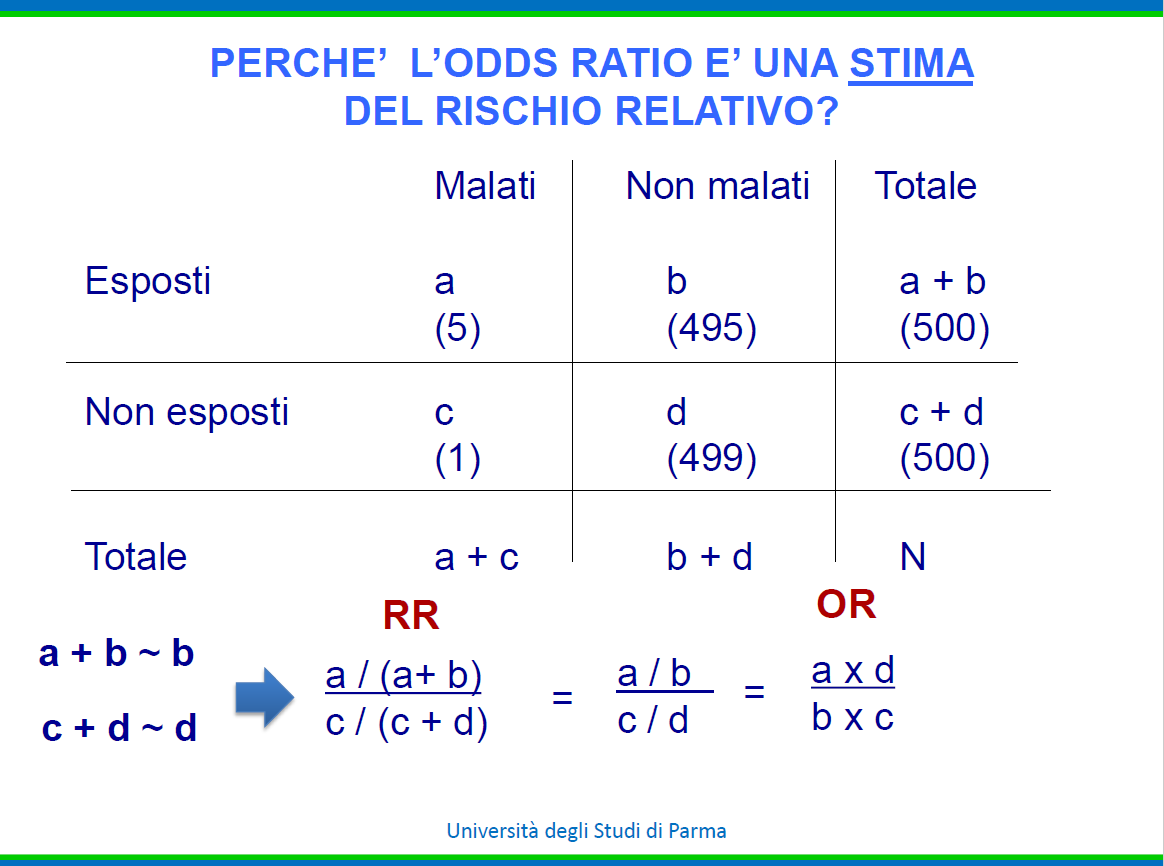
\includegraphics[width=0.8\textwidth]{04/image6.png}
	\end{figure}

L'odds ratio = odds di esposizione nei casi / odds di esposizione nei
controlli

casi: malati esposti/malati non esposti a/c

controlli: controlli esposti/controlli non esposti b/d

quindi odds ratio=a:c / b:d a x d / b x c

\emph{L'odds ratio è una stima del rischio relativo.}

Come si dimostra matematicamente?

Rischio relativo (RR) = a : (a + b) / c : (c + d)

Quindi l'odds ratio è tanto più uguale a RR quanto più (a + b) ha valore
numerico uguale a (b) e allo stesso modo (c + d) è uguale a (d), ovvero
quando i valori (a) e (c) sono bassi in questo modo il risultato sarà
numericamente vicino a quello dell'odds ratio. (vedi figura, uguaglianza
in basso)

Quindi l'odds ratio è tanto più una stima precisa del rischio relativo
quanto più si tratta di una malattia \emph{rara.}

La misura più affidabile è sempre il rischio relativo, ma se non è
disponibile uno studio a coorte, ma solo uno caso-controllo, in cui si
hanno solo il numero degli esposti e dei non esposti in malati e non
malati, allora si calcola l'odds ratio. È tanto più simile al rischio
relativo quanto più la malattia è poco frequente.

Es. primo studio su associazione tra numero di sigarette al giorno e
prevalenza cancro polmone, che era stato fatto proprio su medici.

\begin{figure}[!ht]
\centering
	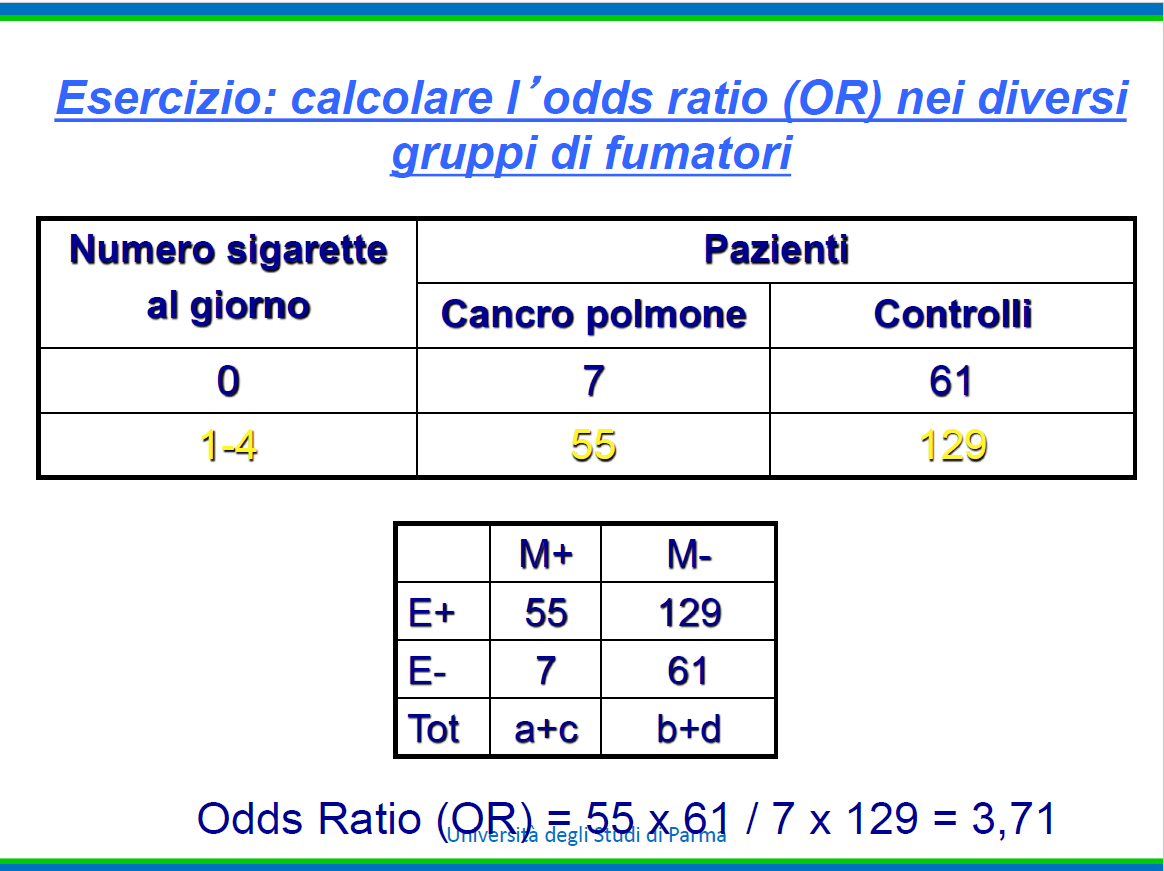
\includegraphics[width=0.8\textwidth]{04/image7.png}
	\end{figure}

Non esposti numero sigarette al giorno= 0; individui con cancro polmone=
7; controlli(sani)= 61

Esposti numero sigarette al giorno= 0-4; individui con cancro polmone=
55; controlli= 129

Quindi 55x61 / 7x129 = 3,71 l'odds ratio di tumore negli esposti è quasi
4 volte maggiore dell'odds di tumore al polmone nei non esposti.

Aumentando esposizione (numero sigarette), aumenta odds ratio patologia:
c'è un effetto dose-risposta.

\subparagraph{Studi Sperimentali}


Negli studi sperimentali si introduce l'esposizione. I più tipici sono i
trials clinici, che valutano l'efficacia di una terapia. Possono essere
trials clinici individuali o anche di comunità.

La maggior parte delle evidenze scientifiche derivano da trials clinici.

\subparagraph{Randomized controller trials }


Si introduce artificialmente un fattore di esposizione, che non è per
forza un fattore di rischio, può anche essere protettivo (ad esempio un
farmaco), in uno solo di due gruppi.

Es. Voglio studiare efficacia di un farmaco oncologico.

Si prende un gruppo di pz oncologici e li si divide in due gruppi: uno a
cui si somministra il trattamento che si vuole studiare e l'altro a cui
non viene somministrato niente oppure viene dato il placebo o un'altra
terapia. Questi gruppi vengono seguiti nel tempo, per un periodo più o
meno lungo di follow up e si valutano i risultati.

Concetto di \textbf{randomizzazione}: l'assegnazione dei pz ai due
gruppi deve essere random, cioè assolutamente casuale, perché i due
gruppi devono essere il più possibile uguali e comparabili e che l'unica
differenza sia nel trattamento, mentre siano uguali per tutte le altre
caratteristiche di età, sesso, comorbidità, ecc... al fine che la
comparazione sia il più possibile oggettiva. Ci sono tecniche di
randomizzazione. Questo limita il più possibile la disomogeneità.

Se questi due gruppi non fossero simili per gravità di patologia, il
rischio sarebbe di avere una sottostima dell'efficacia del trattamento
ad esempio perché si somministra la terapia a pz più gravi.

Caratteristiche:

\begin{itemize}
\item
  sono fatti in condizioni sperimentali
\item
  basso rischio bias e confondimento: sono gli studi ideali, sono quelli
  che più si avvicinano alla verità assoluta, perché lo sperimentatore
  ha la possibilità di introdurre in maniera artificiale l'intervento da
  andare a testare. Sono all'apice della piramide delle evidenze.
\item
  molto complessi
\item
  molto costosi
\item
  aspetti etici: non sempre si può somministrare un trattamento proprio
  per questioni etiche.
\end{itemize}

Gli studi sperimentali sono quelli di approvazione dei farmaci (fase
1,2,3...)

\paragraph{Risultati dei disegni di studio }


I risultati dei disegni di studio vengono \emph{sintetizzati} e
\emph{disseminati} attraverso la letteratura scientifica (i papers) e
costituiscono le \textbf{evidenze scientifiche} sulle quali si basa la
medicina moderna.

Le evidenze scientifiche a cosa servono?

\begin{enumerate}
\def\labelenumi{\arabic{enumi}.}
\item
  a guidare le decisioni cliniche
\item
  ad informare le politiche sanitarie
\end{enumerate}

queste due sono le principali utilità.

\begin{enumerate}
\def\labelenumi{\arabic{enumi}.}
\item
  ad identificare aree dove ulteriori ricerche sono necessarie e quindi
  quesiti di ricerca rilevanti
\item
  ad identificare priorità di ricerca, tematiche, che è prioritario che
  la ricerca approcci
\item
  a sostenere e supportare gli obiettivi di nuovi progetti di ricerca
\item
  interpretare i risultati di un progetto di ricerca
\end{enumerate}

La letteratura scientifica si divide:

\begin{itemize}
\item
  \textbf{primaria}: utilizza dati originali (i disegni di studio)
\item
  \textbf{secondaria}: sintetizza in maniera qualitativa e/o
  quantitativa la letteratura primaria, le evidenze scientifiche
  (metanalisi e revisioni sistematiche).
\item
  \textbf{terziaria}: strumenti per orientare la pratica clinica e le
  politiche sanitarie (utilizzando la letteratura primaria e
  secondaria): linee guida, HTA
\end{itemize}

La letteratura secondaria è fondamentale, perché il numero di evidenze
scientifiche pubblicate su PubMed è enorme e aumenta in maniera
esponenziale.

Le revisioni possono essere narrative e sistematiche. Una
\textbf{revisione narrativa} è un riassunto non sistematico di tutto
quello che viene detto su un argomento; non ha molto valore scientifico
e la sua collocazione sulla piramide delle evidenze non è ai vertici. Le
\textbf{revisioni sistematiche} invece sono ai vertici; sono degli studi
che raccolgono in maniera sistematica e rigorosa tutte le evidenze
disponibili su un determinato argomento.

La \textbf{metanalisi} è l'analisi \emph{quantitativa} di tutte queste
evidenze. La revisione sistematica le raccoglie, la metanalisi le
analizza numericamente. È una tecnica statistica, che mette insieme i
risultati di più studi che hanno approcciato lo stesso argomento.

La revisione sistematica è un tentativo di sintetizzare i risultati di
due o più pubblicazioni su una determinata problematica sanitaria. Viene
realizzata attraverso un approccio scientifico rigoroso ed è un vero e
proprio progetto di ricerca.

Una revisione sistematica può o meno includere una metanalisi. Una
metanalisi è un'analisi statistica dei risultati di studi indipendenti,
che ha generalmente come obiettivo quello di produrre una singola stima
numerica (ad esempio una singola stima di rischio relativo) dell'effetto
di un trattamento, di un intervento.

Es. di metanalisi: impatto del trattamento sulla mortalità espresso come
odds ratio. I diversi studi hanno trovato odds ratio diversi, la
metanalisi consente di mettere numericamente insieme tutti i valori di
odds ratio, tenendo in considerazione anche le dimensioni dei campioni
dei singoli studi, trovando un risultato di odds ratio che li
sintetizza.

Ci sono dei documenti che dicono esattamente quali sono gli step per
fare una revisione sistematica o una metanalisi.

{[}I passi di una revisione sistematica li guardate da soli o saranno
affrontati nella prossima lezione{]}

\begin{figure}[!ht]
\centering
	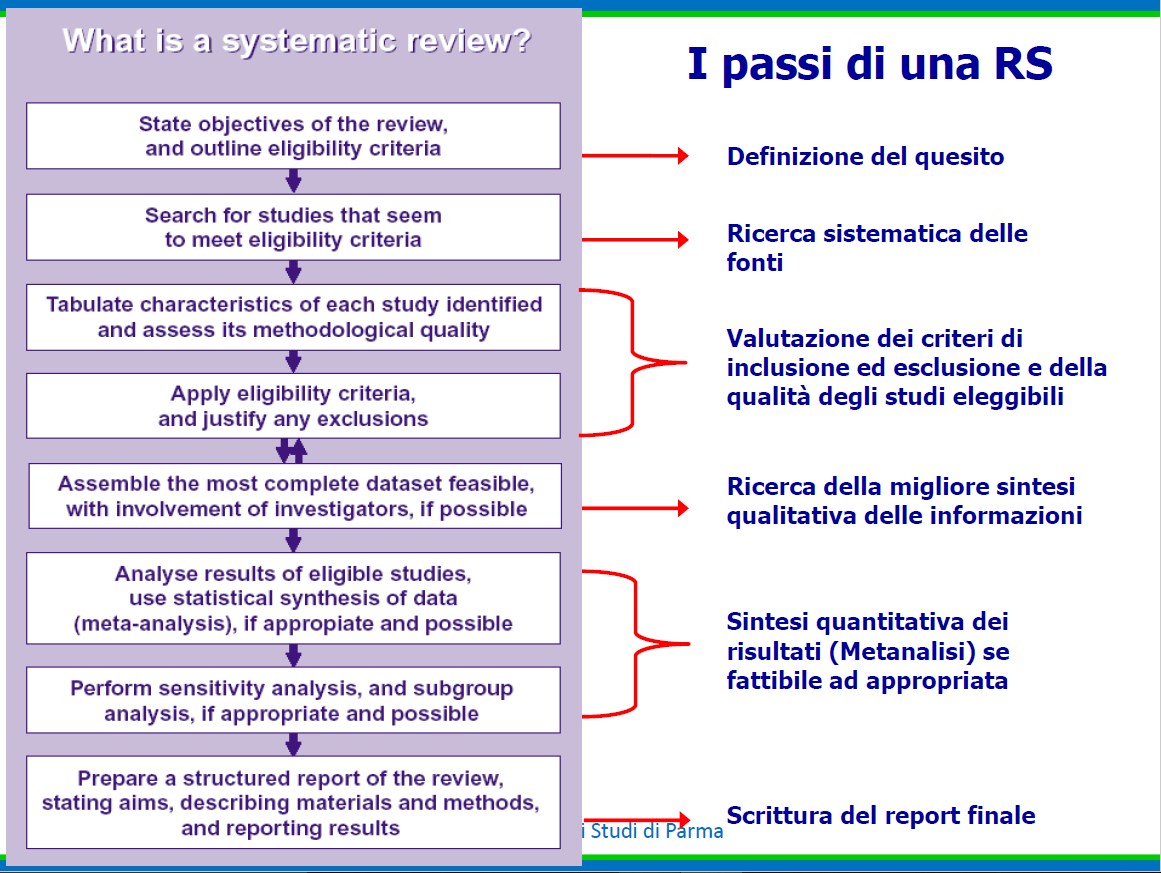
\includegraphics[width=0.8\textwidth]{04/image8.png}
	\end{figure}


{[}Nelle tesi di laurea una revisione sistematica è considerata una
ricerca sperimentale e una metanalisi si può fare anche senza dati, dato
che spesso non sono disponibili, ma se avete un buon quesito di ricerca
potete fare una metanalisi ed è considerata uno studio sperimentale.{]}

